\documentclass{report}
\usepackage{amsfonts,amsthm,amsmath,latexsym}
\usepackage[margin=1.5in]{geometry}
\usepackage{graphicx}
\usepackage[titles,subfigure]{tocloft}
\usepackage{complexity}
\usepackage{scribe-book}
\usepackage{tikz}
\usetikzlibrary{arrows}
\usetikzlibrary{calc,through,backgrounds,decorations.pathmorphing}


\usepackage{caption}
\usepackage{subcaption}
\usepackage{float}

\begin{document}
\newpage
\setcounter{page}{1}
\pagenumbering{roman}  % Roman numbering in intro portion.
\begin{center}
{\bf \Huge Preface}         
\end{center}

\noindent
Matter to be entered here.

\newpage
\listofscribe          % For automatic scribe list generation.

\newpage
\tableofcontents

\setcounter{page}{0}
\pagenumbering{arabic}  % Arabic page numbering for lectures.

\newpage
\def\thislecturealone{1} %

\ifnum\thislecturealone=1
	\documentclass{report}
	\usepackage{amsfonts,amsthm,amsmath,latexsym}
	\usepackage{graphicx,fullpage}
	\usepackage[titles,subfigure]{tocloft}
	\usepackage[margin=1.5in]{geometry}
	\usepackage{complexity}
	\usepackage{scribe-book}
	\usepackage{caption,subcaption,float}
	% *******************************
	% Add packages that you need here
	% *******************************
	\usepackage{tikz}
	\usetikzlibrary{arrows}
	\usetikzlibrary{calc,through,backgrounds,decorations.pathmorphing}
	% *******************************
\fi

% Define custom commands here 
% ****************************
\newcommand{\CYCLE}{{\sf CYCLE~}}
\newcommand{\FPSPACE}{{\sf FPSPACE~}}
\newcommand{\N}{{\mathbb{N}}}
\newcommand{\Z}{{\mathbb{Z}}}
\newcommand{\F}{{\mathbb{F}}}
% ****************************

\ifnum\thislecturealone=1
\begin{document}
\fi

\Lecture{Dinesh K.}{Jan 10, 2012}{4}{Quest for Structure in Counting Problems}
%\theme{Between $\P$ and $\PSPACE$.}
%\lectureplan{Counting problems and their structural complexity. Various attempts to develop the theory and the class $\#\P$. Basic containments.}

%We have seen several decision problems where we are interested in knowing the
%existence or non-existence of objects satisfying a certain property. An
%equally interesting question would be to ask the count of such objects. Such
%problems are called as counting problem.

In the previous lecture, we saw that the counting problem can be as hard as (or 
harder than) the decision problem as given an algorithm for counting problem
the decision problem reduces to just checking the count to be zero or not. We
also saw an easy decision problem \CYCLE whose counting version \#\CYCLE is
\NP-hard (by reduction from {\sf HAMCYCLE}) implying that easy decision
problems can also have corresponding counting problems hard. We also argued
that talking about counting problems still makes sense as the count value,
though exponential, can still be represented in polynomial number of
bits.

In this lecture, we will study counting problems and understand their
structural complexity. We shall also make attempts to develop the theory of
complexity classes capturing the counting problems (especially \#\P). We shall
also discuss their basic containments.

\section{Preliminaries}
Firstly, we fix our computation model where we have a Turing machine with an
input tape, work tape and an output tape. We are interested in the resources
used by the Turing machine - space (considering only the work tape) and time.

We want to capture the notion of counting formally. One such way is to see it
as computing a function $f : \Sigma^* \to \N$ where $\Sigma=\{0,1\}$ which
gives an integer value. So, how can we capture the notion of computing a
function? There are two possible ways of capturing function computation.
\begin{description}
\item[Variant 1] We say that a function $f$ is computable if each bit of the
output can be computed in some decision complexity class $\calC$.
\item[Variant 2] $f$ is computable if the value of the function computation
can be written down within the resource bounds.
\end{description}

Analogous to the decision problems, we define complexity classes for function
computation problems. A natural extension of \P~is \FP~ which is defined as
\begin{center}
\FP = $\{f \left | \right . f:\Sigma^* \to \N, f(x) \text{ for any } x \in
\Sigma^* \text{ can be written down in } poly(|x|) \text{ time}\}$
\end{center}

Now, we shall plugging in the two variants of function computation and see
which of them is more appropriate.

\section{Comparing the variants}
We quickly observe that the first and the second variant really coincides when we are talking
about deterministic computations. Let us do this analysis by attempting the definition of $\FP$.
Following the first variant $f \in \FP$ iff there exists an algorithm that can
compute each bit of $f$ in class \P. But since the algorithm is deterministic, this is  
equivalent to saying that $\forall~i$, the language defined by the $i^{th}$ bit 
$$L_{f_i} = \{ x : (f(x))_i = 1 \} \in \P$$
On the other hand, if each bit can be computed in polynomial time 
and since the count value can be represented in polynomial number of bits, for
evaluation, we just run a polynomial time algorithm polynomial times
which is still a polynomial. Hence we have an algorithm that satisfies the 
second variant.

Hence for deterministic polynomial time computation both variants are equivalent.
We can define other classes for deterministic computation 
like {\sf FL}(log space bounded function computation), \FPSPACE(polynomial
space bounded function computation). Containments of these classes are
analogous to their decision versions. We leave the proof as an exercise.

\begin{lemma}
${\sf FL} \subseteq \FP \subseteq \FPSPACE$
\end{lemma}

Now we turn into the non-deterministic world. 
Following variant 1 of definition of function computation, we must have each
bit computable in class \NP. But variant 2 is not useful because an non-deterministic 
poly time Turing machine by our model is not set to output a value. How can we
capture the function computation for a non-deterministic machine for decision
problems which works by guess-verify mechanism?

Now, consider the non-deterministic algorithm
we had for \SAT, which does guessing of an assignment and verifying it. 
We can observe the following additional property.
\begin{observation}
Number of satisfying assignments is exactly equal to the number of accepting
paths.
\end{observation}
This leads to the question as to whether this is accidental or is there some
hidden structure? It also assigns a function value to the non-deterministic Turing machine.
This motivates us to give a new model, for us to call $f$ is computable by a non-deterministic polynomial time Turing machine.

\begin{definition}
$f$ is $\#\P$ if there exists a non-deterministic Turing machine $M$ running in time $p(n)$ such that 
$\forall x \in \Sigma^*$, $f(x) = \left| \{ y \in \{0,1\}^{p(n)}  : M \textrm{ accepts on path $y$ } \} \right|$.
\end{definition}

\begin{remark}
The RHS is also the number of accepting paths of $M$ on $x$ if the lengths of all paths are equal to $p(n)$.
We remark that this can be achieved without loss of generality. That is, from an arbitrary TM $M$, we can get to a new TM $M'$ which has the same number of accepting paths, such that the number of accepting paths on any input $x$ remains the same. We recall our observation that for length of all non-deterministic paths of an \NP~machine on any input can be made equal without changing the accepted language\footnote{In particular, we showed that a language $A \in \NP$ if and only if there is a language $B \in \P$ and a polynomial $p(n)$ such that $x \in A \iff \exists y \in \{0,1\}^{p(n)} : (x,y) \in B$} . But this construction makes the language accepted the same, and need not keep the number of accepting paths the same. We modify it slightly to achieve our goal.  Indeed, if a path is shorter than $p(n)$ bits and decided A/R, we extend it to the required length using a binary tree of paths rooted at that node and make the left most path (in this binary tree) report A/R respectively and make all other paths reject. The number of accepting paths does not change due to this construction.
\end{remark}

\begin{remark}
Try this as an exercise. Initiate the thought process on : how does this definition compare with variant 1? What does computing/testing each bit to be 0/1 mean?
\end{remark}

%\begin{proof}
%Recall that, 
%\begin{center}
%$ \calL \in \NP \iff \exists \calB \in \P \text{ and a polynomial } p(n)
%\text{ such that} $ 
%$(x \in \calL \iff \exists y \in \{0,1\}^{p(n)}, (x, y) \in \calB )$
%\end{center}
%Hence  a non-deterministic machine $N$ for $\calL$ just need to guess $p(n)$
%bits and run the verifier to validate the guess. Hence every non-deterministic
%path will be of length $p(n)$.
%\end{proof}
%Hence our observation actually follows from the definition. This gives us a
%better characterisation.

%\begin{definition}
%$f$ is computable by a non-deterministic Turing machine $M$ running in 
%ime $p(n)$ if $ \forall x \in \Sigma^*, f(x) = |\{ y \in \{0,1\}^{p(n)} | 
% \text{ accepts on path } y \}|$. The class of functions for which such 
%non-deterministic Turing machines exists is called \#\P (``sharp P")
%\end{definition}

Counting version of \SAT~denoted as \#\SAT~can be defined as 
\[ \#\SAT(\phi) = |\{ \sigma | \phi(\sigma) = 1, \sigma \text{ is a boolean
assignment to variables in } \phi \}| \]
It follows from our observation that $\#\SAT \in \#\P$, since we can give a
non-deterministic machine (i,e. a machine for \SAT) where number of accepting
paths equals to the number of satisfying truth assignments. It can also be
shown that $\#\CYCLE \in \#\P$.

\begin{claim}
$\#\CYCLE \in \#\P$
\end{claim}
\begin{proof}
Following is a non-deterministic Turing machine $N$, such that number of
cycles equals number of accepting paths.

$N$ = `` On input $G$,
\begin{enumerate}
\item Guess subsets $V' \subseteq V(G)$ and $E' \subseteq E(G)$ 
non-deterministically.
\item Accept iff $V', E'$ form a simple cycle. "
\end{enumerate}

Now it follows that $\#\CYCLE(G) = |\{ \# \text{ of accepting paths of } N
\text{ on } G \}|$ since any cycle can uniquely be characterised by an edge set
and a vertex set.
\end{proof}

\section{Basic Containments}
In the functional world, we have the following scenario.
\begin{center}
\FPSPACE \\
$\vert$ \\
\FP \\
$\vert$ \\
{\sf FL }
\end{center}

So where does set of functions, $\#\P$ lie? We will argue that $\#\P$ lies between 
\FP and \FPSPACE thus replicating the picture in the decision world.
\begin{lemma}
$\#\P \subseteq \FPSPACE$
\end{lemma}
\begin{proof}
Given a non-deterministic poly time Turing machine $M$ computing function $f$,
we just need to do a simulation in deterministic poly space. This can be done by
simulating $M$ over all non deterministic paths while reusing space across the
paths. Since length of any path is polynomially bounded, space used will also
be polynomial. In the process we need to keep the count of accepting paths
which can be $\le 2^{p(n)}$ but still representable with $p(n)$ bits in
binary. Hence space requirement is only polynomial in input length.
\end{proof}

\begin{lemma}
$\FP \subseteq \#\P$
\end{lemma}
\begin{proof}
Given an $\calL \in \FP$, there exists a deterministic Turing machine $M$ which
$\forall x \in \calL$ writes $f(x)$ in $p(n)$ time where $p$ is a polynomial
and $n = |x|$. To show that $\calL \in \#\P$, we need to construct a
non-deterministic  such that
\begin{center}
No of accepting paths = $f(x)$.
\end{center}
$N$ can compute $f(x)$ by simulating $M$. Let the value obtained be $k$. Now,
$N$ must have exactly $k$ accepting paths. This can be ensured by guessing
$\lceil \log k \rceil$ bits and accepting all the paths whose address have
binary representations  $\le k$ and rejecting the remaining paths.

$N$ runs in poly time since $f(x)$ computation (simulation of $M$) takes only
polynomial time. Even though $f(x)$ is exponential, number of bits guessed is
$\lceil \log f(x) \rceil$ which will be polynomial in $n$. Hence depth is
polynomially bounded. Also number of accepting paths equals $f(x)$ by
construction. Thus $N'$ is a \#\P machine accepting $\calL$. Hence $\calL =
L(N') \in \#\P$.
\end{proof}

\begin{figure}[htp!]
\centering
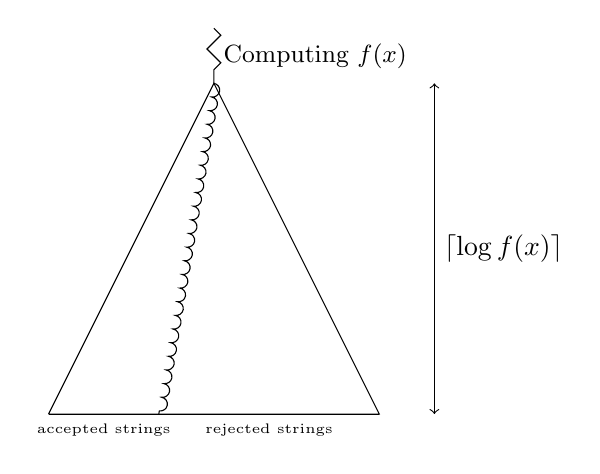
\begin{tikzpicture}[scale=0.7]
\coordinate (T) at (3,7);
\coordinate (A) at (0,0);
\coordinate (B) at (6,0);
\coordinate (C) at (3,6);
\coordinate (M) at (2,0);
\draw [decorate,decoration=zigzag] (T) -> (C) node[midway,right]
{ {\small Computing $f(x)$ }};
\draw (A) -- (M) node[midway,below] { {\tiny accepted strings}} ;
\draw (M) -- (B) node[midway,below] { {\tiny rejected strings}} ;
\draw (A) -- (B) -- (C) -- (A);
\draw [decorate,decoration=bumps] (C) -> (M);
\draw [<->] (7,0) -- (7,6) node[midway,right] {$\lceil \log f(x) \rceil$};
\end{tikzpicture}
\end{figure}

It can be observed that if function computation can be done in polynomial time
then $\P = \NP$. This is because solving decision problem amounts to checking
if the corresponding counting function gives a non zero value or not hence
making decision problem easy if function computation is in \P. 
\begin{lemma}
$\#\P = \FP \implies \P = \NP$
\end{lemma}

An interesting question would be to ask if the converse it true? That is 
\begin{center}
Does $\P = \NP \text{ imply }  \#\P = \FP ?$
\end{center}
We will address this and show a weaker implication (that is, based on slightly stronger LHS) in the next lecture.


\ifnum\thislecturealone=1
\end{document}
\fi


\documentclass[11pt]{article}
\usepackage{amsmath,amssymb,amsfonts,amsthm,complexity}

\newcommand{\CYCLE}{{\sf CYCLE~}}
\newcommand{\FPSPACE}{{\sf FPSPACE~}}
\usepackage{tikz}
\usetikzlibrary{calc,through,backgrounds,decorations.pathmorphing}

%%%%%%%%%%%%%%%%%%%%%%%%%%%%%%%%%%%%%%%%%%%%%%%%%%%%%%
%
% This file should be called  preamble.tex 
% Your main LaTeX file should look like :
%
%	\documentclass[11pt]{article}
%	\usepackage{amsmath,amssymb,amsfonts,amsthm,complexity}
%
%	%%%%%%%%%%%%%%%%%%%%%%%%%%%%%%%%%%%%%%%%%%%%%%%%%%%%%%
%
% This file should be called  preamble.tex 
% Your main LaTeX file should look like :
%
%	\documentclass[11pt]{article}
%	\usepackage{amsmath,amssymb,amsfonts,amsthm,complexity}
%
%	\input{preamble.tex}
%	\begin{document}
%
%	\lecture{LECTURE NO.}{TITLE OF SCRIBE}{DATE}{Jayalal Sarma M.N.}{YOUR NAME}
%	\theme{THEME FOCUS}
%	\lectureplan{A BRIEF DESCRIPTION OF THE LECTURE}
%	
%	\section{TOPIC 1}
%	...
%	\section{TOPIC 2}
% 	...
%	\end{document}
% If there is not title, leave it as {}
 

\newtheorem{theorem}{Theorem}
\newtheorem{corollary}[theorem]{Corollary}
\newtheorem{lemma}[theorem]{Lemma}
\newtheorem{observation}[theorem]{Observation}
\newtheorem{proposition}[theorem]{Proposition}
\newtheorem{claim}[theorem]{Claim}
\newtheorem{fact}[theorem]{Fact}
\newtheorem{example}[theorem]{Example}
\newtheorem{assumption}[theorem]{Assumption}

\theoremstyle{definition}
\newtheorem{definition}[theorem]{Definition}

\theoremstyle{remark}
\newtheorem{remark}[theorem]{Remark}

% Setting theorem style back for theorems defined in main file.
\theoremstyle{plain}

%\newenvironment{proof}{\noindent{\bf Proof}\hspace*{1em}}{\qed\bigskip}
\newenvironment{proof-sketch}{\noindent{\bf Sketch of Proof}\hspace*{1em}}{\qed\bigskip}
\newenvironment{proof-idea}{\noindent{\bf Proof Idea}\hspace*{1em}}{\qed\bigskip}
\newenvironment{proof-of-lemma}[1]{\noindent{\bf Proof of Lemma #1}\hspace*{1em}}{\qed\bigskip}
\newenvironment{proof-attempt}{\noindent{\bf Proof Attempt}\hspace*{1em}}{\qed\bigskip}
\newenvironment{proofof}[1]{\noindent{\bf Proof}
of #1:\hspace*{1em}}{\qed\bigskip}

%%%%%%%%%%%%%%%%%%%%%%%%%%%%%%%%%%%%%%%%%%%%%%%%%%%
% Useful Complexity Classes
%%%%%%%%%%%%%%%%%%%%%%%%%%%%%%%%%%%%%%%%%%%%%%%%%%%
\newcommand{\ntime}{\hbox{NTIME}}
\newcommand{\nspace}{\hbox{NSPACE}}
\newcommand{\conspace}{\hbox{co-NSPACE}}
\newcommand{\np}{\hbox{NP}}
\newcommand{\pspace}{\hbox{PSPACE}}
\newcommand{\lspace}{\hbox{L}}
\newcommand{\conp}{\hbox{coNP}}
\newcommand{\exptime}{\hbox{EXPTIME}}
\newcommand{\elem}{\hbox{E}}
\newcommand{\nl}{\hbox{NL}}
\newcommand{\bpp}{\hbox{BPP}}
\newcommand{\nregexp}{\hbox{NREGEXP}}
\newcommand{\tqbf}{\hbox{TQBF}}
\newcommand{\threesat}{\hbox{3SAT}}
\newcommand{\cvp}{\hbox{CVP}}
\newcommand{\stconn}{\hbox{STCONN}}
\newcommand{\ispath}{\hbox{ISPATH}}

%\newcommand{\class}{\hbox{$\mathbb{C}$}} 
%\newcommand{\class}{\hbox{$\mathbf{C}$}} 

\newcommand{\lep}{\leq _{\hbox{P}}}
\newcommand{\lel}{\leq _{\hbox{L}}}
\newcommand{\aspace}[1]{{\rm ASPACE}(#1)}
\newcommand{\atime}[1]{{\rm ATIME}(#1)}
\newcommand{\dtime}[1]{{\rm DTIME}(#1)}
\newcommand{\spa}[1]{{\rm SPACE}(#1)}
\newcommand{\ti}[1]{{\rm TIME}(#1)}
\newcommand{\ap}{{\rm AP}}
\newcommand{\al}{{\rm AL}}


%%%%%%%%%%%%%%%%%%%%%%%%%%%%%%%%%%%%%%%%%%%%%%%%%%%
% Useful Macros
%%%%%%%%%%%%%%%%%%%%%%%%%%%%%%%%%%%%%%%%%%%%%%%%%%%
\renewcommand{\Pr}[1]{\mathify{\mbox{Pr}\left[#1\right]}}
\newcommand{\Exp}[1]{\mathify{\mbox{Exp}\left[#1\right]}}
\newcommand{\bigO}O
\newcommand{\set}[1]{\mathify{\left\{ #1 \right\}}}
\def\half{\frac{1}{2}}

\def\implies{\Rightarrow}
\def\prob#1#2{{\mathop{{\rm Prob}}_{#1}}\left[#2 \right]}
\def\var#1#2{{\mathop{{\rm Var}}_{#1}}[#2]}
\def\expec#1#2{{\mathop{{\rm E}}_{#1}}[#2]}
\def\sizeof#1{\left| #1\right|}
\def\setof#1{\left\{ #1\right\}  }

\newcommand{\F}{{\mathbb{F}}}
\newcommand{\Z}{{\mathbb{Z}}}
\newcommand{\N}{\mathbb{N}}
%\newcommand{\qed}{\rule{7pt}{7pt}}

% \makeatletter
% \@addtoreset{figure}{section}
% \@addtoreset{table}{section}
% \@addtoreset{equation}{section}
% \makeatother

\newcommand{\FOR}{{\bf for}}
\newcommand{\TO}{{\bf to}}
\newcommand{\DO}{{\bf do}}
\newcommand{\WHILE}{{\bf while}}
\newcommand{\AND}{{\bf and}}
\newcommand{\IF}{{\bf if}}
\newcommand{\THEN}{{\bf then}}
\newcommand{\ELSE}{{\bf else}}

% \renewcommand{\thefigure}{\thesection.\arabic{figure}}
% \renewcommand{\thetable}{\thesection.\arabic{table}}
% \renewcommand{\theequation}{\thesection.\arabic{equation}}

% Calligraphic letters
\newcommand{\calA}{{\cal A}}
\newcommand{\calB}{{\cal B}}
\newcommand{\calC}{{\cal C}}
\newcommand{\calD}{{\cal D}}
\newcommand{\calE}{{\cal E}}
\newcommand{\calF}{{\cal F}}
\newcommand{\calG}{{\cal G}}
\newcommand{\calH}{{\cal H}}
\newcommand{\calI}{{\cal I}}
\newcommand{\calJ}{{\cal J}}
\newcommand{\calK}{{\cal K}}
\newcommand{\calL}{{\cal L}}
\newcommand{\calM}{{\cal M}}
\newcommand{\calN}{{\cal N}}
\newcommand{\calO}{{\cal O}}
\newcommand{\calP}{{\cal P}}
\newcommand{\calQ}{{\cal Q}}
\newcommand{\calR}{{\cal R}}
\newcommand{\calS}{{\cal S}}
\newcommand{\calT}{{\cal T}}
\newcommand{\calU}{{\cal U}}
\newcommand{\calV}{{\cal V}}
\newcommand{\calW}{{\cal W}}
\newcommand{\calX}{{\cal X}}
\newcommand{\calY}{{\cal Y}}
\newcommand{\calZ}{{\cal Z}}


% Some macro's from Speilman's course.

\makeatletter
\def\fnum@figure{{\bf Figure \thefigure}}
\def\fnum@table{{\bf Table \thetable}}
\long\def\@mycaption#1[#2]#3{\addcontentsline{\csname
  ext@#1\endcsname}{#1}{\protect\numberline{\csname 
  the#1\endcsname}{\ignorespaces #2}}\par
  \begingroup
    \@parboxrestore
    \small
    \@makecaption{\csname fnum@#1\endcsname}{\ignorespaces #3}\par
  \endgroup}
\def\mycaption{\refstepcounter\@captype \@dblarg{\@mycaption\@captype}}
\makeatother

\newcommand{\figcaption}[1]{\mycaption[]{#1}}
\newcommand{\tabcaption}[1]{\mycaption[]{#1}}


%%%%%%%%%%%%%%%%%%%%%%%%%%%%%%%%%%%%%%%%%%%%%%%%%%%%%%%%%%%%%%%%%%%%%%
% Feel free to ignore the rest of this file.

%%%%%%%%%%%%%%%%%%%%%%%%%%%%%%%
% Margins and page indentations
% DO NOT EDIT
%%%%%%%%%%%%%%%%%%%%%%%%%%%%%%
\textwidth=6in
\oddsidemargin=0.25in
\evensidemargin=0.25in
\topmargin=-0.1in
\footskip=0.8in
\parindent=0.0cm
\parskip=0.3cm
\textheight=8.00in
\setcounter{tocdepth} {3}
\setcounter{secnumdepth} {2}
\sloppy


\newcommand{\handout}[5]{
   \renewcommand{\thepage}{#1-\arabic{page}}
   \noindent
   \begin{center}
   \framebox{
      \vbox{
    \hbox to 5.78in { {\bf CS6840: Advanced Complexity Theory} \hfill #2 }
       \vspace{4mm}
       \hbox to 5.78in { {\Large \hfill #5  \hfill} }
       \vspace{2mm}
       \hbox to 5.78in { {\em #3 \hfill #4} }
      }
   }
   \end{center}
   \vspace*{4mm}
}

\newcommand{\lecture}[5]{\handout{#1}{#3}{Lecturer:~#4}{Scribe: #5}{Lecture~#1~: #2}}

\newcommand{\lectureplan}[1]{{\sc Lecture Plan:}#1\\}
\newcommand{\theme}[1]{{\sc Theme:} #1\\}

%	\begin{document}
%
%	\lecture{LECTURE NO.}{TITLE OF SCRIBE}{DATE}{Jayalal Sarma M.N.}{YOUR NAME}
%	\theme{THEME FOCUS}
%	\lectureplan{A BRIEF DESCRIPTION OF THE LECTURE}
%	
%	\section{TOPIC 1}
%	...
%	\section{TOPIC 2}
% 	...
%	\end{document}
% If there is not title, leave it as {}
 

\newtheorem{theorem}{Theorem}
\newtheorem{corollary}[theorem]{Corollary}
\newtheorem{lemma}[theorem]{Lemma}
\newtheorem{observation}[theorem]{Observation}
\newtheorem{proposition}[theorem]{Proposition}
\newtheorem{claim}[theorem]{Claim}
\newtheorem{fact}[theorem]{Fact}
\newtheorem{example}[theorem]{Example}
\newtheorem{assumption}[theorem]{Assumption}

\theoremstyle{definition}
\newtheorem{definition}[theorem]{Definition}

\theoremstyle{remark}
\newtheorem{remark}[theorem]{Remark}

% Setting theorem style back for theorems defined in main file.
\theoremstyle{plain}

%\newenvironment{proof}{\noindent{\bf Proof}\hspace*{1em}}{\qed\bigskip}
\newenvironment{proof-sketch}{\noindent{\bf Sketch of Proof}\hspace*{1em}}{\qed\bigskip}
\newenvironment{proof-idea}{\noindent{\bf Proof Idea}\hspace*{1em}}{\qed\bigskip}
\newenvironment{proof-of-lemma}[1]{\noindent{\bf Proof of Lemma #1}\hspace*{1em}}{\qed\bigskip}
\newenvironment{proof-attempt}{\noindent{\bf Proof Attempt}\hspace*{1em}}{\qed\bigskip}
\newenvironment{proofof}[1]{\noindent{\bf Proof}
of #1:\hspace*{1em}}{\qed\bigskip}

%%%%%%%%%%%%%%%%%%%%%%%%%%%%%%%%%%%%%%%%%%%%%%%%%%%
% Useful Complexity Classes
%%%%%%%%%%%%%%%%%%%%%%%%%%%%%%%%%%%%%%%%%%%%%%%%%%%
\newcommand{\ntime}{\hbox{NTIME}}
\newcommand{\nspace}{\hbox{NSPACE}}
\newcommand{\conspace}{\hbox{co-NSPACE}}
\newcommand{\np}{\hbox{NP}}
\newcommand{\pspace}{\hbox{PSPACE}}
\newcommand{\lspace}{\hbox{L}}
\newcommand{\conp}{\hbox{coNP}}
\newcommand{\exptime}{\hbox{EXPTIME}}
\newcommand{\elem}{\hbox{E}}
\newcommand{\nl}{\hbox{NL}}
\newcommand{\bpp}{\hbox{BPP}}
\newcommand{\nregexp}{\hbox{NREGEXP}}
\newcommand{\tqbf}{\hbox{TQBF}}
\newcommand{\threesat}{\hbox{3SAT}}
\newcommand{\cvp}{\hbox{CVP}}
\newcommand{\stconn}{\hbox{STCONN}}
\newcommand{\ispath}{\hbox{ISPATH}}

%\newcommand{\class}{\hbox{$\mathbb{C}$}} 
%\newcommand{\class}{\hbox{$\mathbf{C}$}} 

\newcommand{\lep}{\leq _{\hbox{P}}}
\newcommand{\lel}{\leq _{\hbox{L}}}
\newcommand{\aspace}[1]{{\rm ASPACE}(#1)}
\newcommand{\atime}[1]{{\rm ATIME}(#1)}
\newcommand{\dtime}[1]{{\rm DTIME}(#1)}
\newcommand{\spa}[1]{{\rm SPACE}(#1)}
\newcommand{\ti}[1]{{\rm TIME}(#1)}
\newcommand{\ap}{{\rm AP}}
\newcommand{\al}{{\rm AL}}


%%%%%%%%%%%%%%%%%%%%%%%%%%%%%%%%%%%%%%%%%%%%%%%%%%%
% Useful Macros
%%%%%%%%%%%%%%%%%%%%%%%%%%%%%%%%%%%%%%%%%%%%%%%%%%%
\renewcommand{\Pr}[1]{\mathify{\mbox{Pr}\left[#1\right]}}
\newcommand{\Exp}[1]{\mathify{\mbox{Exp}\left[#1\right]}}
\newcommand{\bigO}O
\newcommand{\set}[1]{\mathify{\left\{ #1 \right\}}}
\def\half{\frac{1}{2}}

\def\implies{\Rightarrow}
\def\prob#1#2{{\mathop{{\rm Prob}}_{#1}}\left[#2 \right]}
\def\var#1#2{{\mathop{{\rm Var}}_{#1}}[#2]}
\def\expec#1#2{{\mathop{{\rm E}}_{#1}}[#2]}
\def\sizeof#1{\left| #1\right|}
\def\setof#1{\left\{ #1\right\}  }

\newcommand{\F}{{\mathbb{F}}}
\newcommand{\Z}{{\mathbb{Z}}}
\newcommand{\N}{\mathbb{N}}
%\newcommand{\qed}{\rule{7pt}{7pt}}

% \makeatletter
% \@addtoreset{figure}{section}
% \@addtoreset{table}{section}
% \@addtoreset{equation}{section}
% \makeatother

\newcommand{\FOR}{{\bf for}}
\newcommand{\TO}{{\bf to}}
\newcommand{\DO}{{\bf do}}
\newcommand{\WHILE}{{\bf while}}
\newcommand{\AND}{{\bf and}}
\newcommand{\IF}{{\bf if}}
\newcommand{\THEN}{{\bf then}}
\newcommand{\ELSE}{{\bf else}}

% \renewcommand{\thefigure}{\thesection.\arabic{figure}}
% \renewcommand{\thetable}{\thesection.\arabic{table}}
% \renewcommand{\theequation}{\thesection.\arabic{equation}}

% Calligraphic letters
\newcommand{\calA}{{\cal A}}
\newcommand{\calB}{{\cal B}}
\newcommand{\calC}{{\cal C}}
\newcommand{\calD}{{\cal D}}
\newcommand{\calE}{{\cal E}}
\newcommand{\calF}{{\cal F}}
\newcommand{\calG}{{\cal G}}
\newcommand{\calH}{{\cal H}}
\newcommand{\calI}{{\cal I}}
\newcommand{\calJ}{{\cal J}}
\newcommand{\calK}{{\cal K}}
\newcommand{\calL}{{\cal L}}
\newcommand{\calM}{{\cal M}}
\newcommand{\calN}{{\cal N}}
\newcommand{\calO}{{\cal O}}
\newcommand{\calP}{{\cal P}}
\newcommand{\calQ}{{\cal Q}}
\newcommand{\calR}{{\cal R}}
\newcommand{\calS}{{\cal S}}
\newcommand{\calT}{{\cal T}}
\newcommand{\calU}{{\cal U}}
\newcommand{\calV}{{\cal V}}
\newcommand{\calW}{{\cal W}}
\newcommand{\calX}{{\cal X}}
\newcommand{\calY}{{\cal Y}}
\newcommand{\calZ}{{\cal Z}}


% Some macro's from Speilman's course.

\makeatletter
\def\fnum@figure{{\bf Figure \thefigure}}
\def\fnum@table{{\bf Table \thetable}}
\long\def\@mycaption#1[#2]#3{\addcontentsline{\csname
  ext@#1\endcsname}{#1}{\protect\numberline{\csname 
  the#1\endcsname}{\ignorespaces #2}}\par
  \begingroup
    \@parboxrestore
    \small
    \@makecaption{\csname fnum@#1\endcsname}{\ignorespaces #3}\par
  \endgroup}
\def\mycaption{\refstepcounter\@captype \@dblarg{\@mycaption\@captype}}
\makeatother

\newcommand{\figcaption}[1]{\mycaption[]{#1}}
\newcommand{\tabcaption}[1]{\mycaption[]{#1}}


%%%%%%%%%%%%%%%%%%%%%%%%%%%%%%%%%%%%%%%%%%%%%%%%%%%%%%%%%%%%%%%%%%%%%%
% Feel free to ignore the rest of this file.

%%%%%%%%%%%%%%%%%%%%%%%%%%%%%%%
% Margins and page indentations
% DO NOT EDIT
%%%%%%%%%%%%%%%%%%%%%%%%%%%%%%
\textwidth=6in
\oddsidemargin=0.25in
\evensidemargin=0.25in
\topmargin=-0.1in
\footskip=0.8in
\parindent=0.0cm
\parskip=0.3cm
\textheight=8.00in
\setcounter{tocdepth} {3}
\setcounter{secnumdepth} {2}
\sloppy


\newcommand{\handout}[5]{
   \renewcommand{\thepage}{#1-\arabic{page}}
   \noindent
   \begin{center}
   \framebox{
      \vbox{
    \hbox to 5.78in { {\bf CS6840: Advanced Complexity Theory} \hfill #2 }
       \vspace{4mm}
       \hbox to 5.78in { {\Large \hfill #5  \hfill} }
       \vspace{2mm}
       \hbox to 5.78in { {\em #3 \hfill #4} }
      }
   }
   \end{center}
   \vspace*{4mm}
}

\newcommand{\lecture}[5]{\handout{#1}{#3}{Lecturer:~#4}{Scribe: #5}{Lecture~#1~: #2}}

\newcommand{\lectureplan}[1]{{\sc Lecture Plan:}#1\\}
\newcommand{\theme}[1]{{\sc Theme:} #1\\}

\begin{document}
\lecture{5}{\FP vs $\#\P$ question}{Jan 12, 2012}{ Jayalal Sarma M.N.}{Prasun Kumar}
\theme{Between $\P$ and $\PSPACE$.}
\lectureplan{\FP vs $\#\P$ question, a counter part in the decision world. The class PP. PP vs P is equivalent to FP vs $\#\P$.}

We know $(\#\P = \FP) \implies (\P = \NP)$\\
Is the converse also true, i.e., does $(\P = \NP) \implies (\#\P = \FP)$ ?
With this question we ended the last lecture. Interestingly, the status of this
question is still unknown.

In this lecture, we will define a new class of languages \PP(probabilistic polynomial)
in decisoon world and then try to answer the above question by considering the 
containment relationship between the classes \PP and \NP. 


\section{Complexity Class \PP}
With respect to a nondeterministic Turing machine(NTM), we have two different
classes of languages as follows, which differs in their acceptance conditions by NTM 

(i) \NP = $\{$L $|\exists$ NTM $M_1$, x $\in$ L $\iff M_1$ has atleast one accepting path on x $\}$\\
(ii)\coNP = $\{$L $|\exists$ NTM $M_2$, x $\in$ L $\iff$all paths in $M_2$ are accepting paths on x $\}$

So, in terms of number of accepting paths on input {\em x}, we are talking of
extremums. On one side, in \NP  we talk of atleast one accepting path, and on
the other side, in \coNP  we talk of all accepting paths. So here we can ask a
question that will we get a different class of languages if we have larger than some fraction 
of total number of paths as accepting paths by a nondeterministic turing machine
on input {\em x}. The answer to this question is affirmative if we have this fraction
to be half and the corresponding class of languages is called \PP (probabilistic polynomial)
which is defined as follows \\ 

\PP =$\{$L $|\exists$ NTM $M$, x $\in$ L $\iff$ atleast half of the total number of paths are accepting paths on x $\}$

\begin{claim}
 \coNP $\subseteq$ \PP
\end{claim}
\begin{proof}
 directly follows from the definition.
\end{proof}

\begin{claim}
  \NP $\subseteq$ \PP
\end{claim}
\begin{proof}
Let L $\in$  \NP  via a nondeterministic turing machine M,  x $\in$ L $\iff$M has atleast one accepting path on x. 
Our aim is to give another turing machine $M^{'}$ for the same language L such that
x $\in$ L $\iff M^{'}$ has more than half of the total number of paths as accepting paths on x.\\
Description of $M^{'}$ :\\ (i)  simulate M on {\em x}\\
                        (ii) if M accepts then choose one bit nondeterministically and accept in both branches.\\
                       (iii)if M rejects then choose one bit nondeterministically,accept in one branch
                            and reject in other.\\
Assume the height of computation tree of M on {\em x} is $p(n)$. Now, whenever x $\in$ L, number of
accepting paths of $M^{'}$ on {\em x} is $\ge 2^{p(n)}$ where total number of paths in computation tree
for $M^{'}$ is $2^{p(n)+1}$. Whenever x $\not\in$ L,all paths reject in M thus  number of accepting and rejecting
paths in computation tree for $M^{'}$ are same and is equal to $2^{p(n)}$.
\end{proof}
Now, we have the following containment relationship among different classes of languages
 
\begin{center}
\PSPACE \\ 
$\vert$ \\
\PP \\
$\vert$ \\
\NP \\
$\vert$ \\
\P
\end{center}

\begin{theorem}
 $(\#\P = \FP) \iff (\PP = \P)$
\end{theorem}
\begin{proof}
($\Rightarrow$) Assume $\#\P = \FP$, our aim is to prove $\PP = \P$. Equivalently we have to prove that\\
(i) $\P \subseteq \PP$ : it directly follows from the basic containment relation.\\
(ii)$\PP \subseteq \P$ : so we need to show that $(L \in \PP) \implies (L \in \P)$.\\
Let $L \in \PP$ via a NTM M $\implies x \in L$ if and only if more than half of the paths are accepting
paths. Define $\# accept_M(x)$ as the {\em number of accepting paths of M on x}. Now let $f(x)=\# accept_M(x)$
on any input x then $f \in \#p$(by definition). So, $f \in \FP$(by our assumption) thus we can write $f(x)$
in poly time and by checking its value in poly time we can decide whether $x \in L$ or not. So, $L \in \P$.\\

($\Leftarrow$)Assume $\PP = \P$, our aim is to prove $\#\P = \FP$. Equivalently we have to prove that\\
(i) $\FP \subseteq \#\P$ : it directly follows from the basic containment relation.\\
(ii)$\#\P \subseteq \FP$ : so we need to show that $(f \in \#\P) \implies (f \in \FP)$.\\
Let $f\in \#\P$ via a NTM $M$ such that $\forall x$ $f(x)=\# accept_M(x)$. The naive approach
to compute $f(x)$ is to compute the number of accepting paths in computation tree of height $p(n)$ which 
will take exponential time. So we use an alternative way to show that $f \in \FP$ by finding 
the minimum value of $k$ such that $k+\# accept_M(x)\textgreater 2^{p(n)}$. Our aim has now shifted to 
given a $k$,how to figure out $k+\# accept_M(x)\textgreater 2^{p(n)}$. For this, we construct an another 
nondeterministic turing machine $N$ as follows\\
(a){\em Construct a NTM $M^{'}$ having exactly $k$ number of accepting states.}\\

We can always construct such $M^{'}$ by making first lexicographic $k$ paths as accepting paths
and make remaining as rejecting paths.\\

(b){\em Extend the depth of $M^{'}$ from $\log(k)$ to $p(n)$ keeping the number of accepting paths same.}\\

This we can do by making the computation tree a full and complete binary tree of depth $p(n)$. In the
process, for all accepting paths with depth $\le p(n)$ we introduce a subtree at the corresponding leaf 
such that we get a full and complete binary tree and in all those subtrees make the lexicographic first
(leftmost) path as accepting path and make remaining as rejacting paths. Similarly,for all rejecting paths
with depth $\le p(n)$ make all the paths in the subtree as rejecting paths.\

(c)Introduce a new root node which goes to root of computation tree of $M$ on input $0$ and on input $1$
it goes to root of computation tree of $M^{'}$.\
 
Thus it runs in $p(n)+1$ depth and $\# accept_N(x)=k+\# accept_M(x)$.
%Now $\# accept_N(x)= k+\# accept_M(x)\ge 2^{p(n)}$=1\2* $ 2^{p(n)+1}$=(1\2)*{\em total number of paths in
%computation tree of N on x}. So, $x\in L(N)\iff \# accept_N(x)\ge2^{p(n)$. Thus,$L(N)\in \PP\implies L(N)\in \P$
(by our assumption). We are interested in minimum $K$ and $0\le K \le 2^{p(n)}$, so we can make at most $p(n)$
calls to find minimum $K$. So, we can write down $f(x)$ in poly time , hence $f\in\FP$.

\end{proof}



\end{document}


\bibliographystyle{abbrv}
\bibliography{references}

\end{document}
